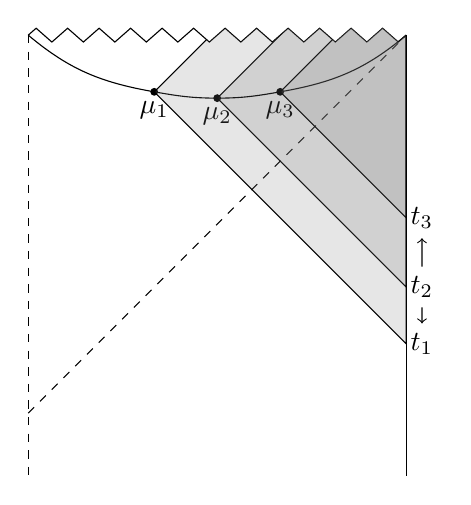
\begin{tikzpicture}[scale=0.8]

  \coordinate (bl) at (0, 0);
  \coordinate (tl) at (0, 7);
  \coordinate (tr) at (6, 7);
  \coordinate (br) at (6, 0);

  \coordinate (ehb) at (0, 1);

  \coordinate (mu1) at (2, 6.1);

  \coordinate[label=below:$\mu_2$] (mu2) at (3, 6);
  \coordinate (owbr2) at (6, 3);
  \node[xshift=0.2cm] (t2) at (owbr2){$t_2$};
  \coordinate (owtr2) at (6 ,9);

  \coordinate (mu3) at (4, 6.1);


  \begin{scope}[decoration={zigzag, segment length=0.4cm}]


    \draw[decorate] (tr) to (tl);
    \draw[dashed] (tl) to (bl);
    \draw[dashed] (ehb) to (tr);
    \draw (tr) to (br);

    \path[clip] (tl) decorate {to (tr)} to (br) to (bl) -- cycle;

    \node at (mu2)[circle,fill,inner sep=1pt]{};

    \draw[fill=gray, fill opacity=0.2] (mu2) to (owtr2) to (owbr2) to (mu2);
  \end{scope} 


  \onslide<2->{
    \draw (tl) to[out=-40, in=170] (mu1) to[out=-10,in=180] (mu2) to[out=0, in=-170] (mu3) to[out=10, in=-140] (tr);
  }

  \onslide<3->{
    \coordinate (owbr3) at (6, 4.1);
    \node[xshift=0.2cm] (t3) at (owbr3){$t_3$};
    \coordinate (owtr3) at (6 ,8.1);
    \begin{scope}[decoration={zigzag, segment length=0.4cm}]
      \path[clip] (tl) decorate {to (tr)} to (br) to (bl) -- cycle;

      \coordinate[label=below:$\mu_3$] (0) at (mu3);
      \node at (mu3)[circle,fill,inner sep=1pt]{};

      \draw[fill=gray, fill opacity=0.2] (mu3) to (owtr3) to (owbr3) to (mu3);
    \end{scope} 
  }
  
  \onslide<5>{
    \draw[->] (t2) to (t3);
  }

  \onslide<6->{
    \coordinate (owbr1) at (6, 2.1);
    \node[xshift=0.2cm] (t1) at (owbr1){$t_1$};
    \coordinate (owtr1) at (6 ,10.1);
    \begin{scope}[decoration={zigzag, segment length=0.4cm}]
      \path[clip] (tl) decorate {to (tr)} to (br) to (bl) -- cycle;

      \coordinate[label=below:$\mu_1$] (0) at (mu1);
      \node at (mu1)[circle,fill,inner sep=1pt]{};

      \draw[fill=gray, fill opacity=0.2] (mu1) to (owtr1) to (owbr1) to (mu1);
    \end{scope} 
    \draw[->] (t2) to (t1);
  }


\end{tikzpicture}
